% Options for packages loaded elsewhere
% Options for packages loaded elsewhere
\PassOptionsToPackage{unicode}{hyperref}
\PassOptionsToPackage{hyphens}{url}
\PassOptionsToPackage{dvipsnames,svgnames,x11names}{xcolor}
%
\documentclass[
]{interact}
\usepackage{xcolor}
\usepackage{amsmath,amssymb}
\setcounter{secnumdepth}{5}
\usepackage{iftex}
\ifPDFTeX
  \usepackage[T1]{fontenc}
  \usepackage[utf8]{inputenc}
  \usepackage{textcomp} % provide euro and other symbols
\else % if luatex or xetex
  \usepackage{unicode-math} % this also loads fontspec
  \defaultfontfeatures{Scale=MatchLowercase}
  \defaultfontfeatures[\rmfamily]{Ligatures=TeX,Scale=1}
\fi
\usepackage{lmodern}
\ifPDFTeX\else
  % xetex/luatex font selection
\fi
% Use upquote if available, for straight quotes in verbatim environments
\IfFileExists{upquote.sty}{\usepackage{upquote}}{}
\IfFileExists{microtype.sty}{% use microtype if available
  \usepackage[]{microtype}
  \UseMicrotypeSet[protrusion]{basicmath} % disable protrusion for tt fonts
}{}
% Make \paragraph and \subparagraph free-standing
\makeatletter
\ifx\paragraph\undefined\else
  \let\oldparagraph\paragraph
  \renewcommand{\paragraph}{
    \@ifstar
      \xxxParagraphStar
      \xxxParagraphNoStar
  }
  \newcommand{\xxxParagraphStar}[1]{\oldparagraph*{#1}\mbox{}}
  \newcommand{\xxxParagraphNoStar}[1]{\oldparagraph{#1}\mbox{}}
\fi
\ifx\subparagraph\undefined\else
  \let\oldsubparagraph\subparagraph
  \renewcommand{\subparagraph}{
    \@ifstar
      \xxxSubParagraphStar
      \xxxSubParagraphNoStar
  }
  \newcommand{\xxxSubParagraphStar}[1]{\oldsubparagraph*{#1}\mbox{}}
  \newcommand{\xxxSubParagraphNoStar}[1]{\oldsubparagraph{#1}\mbox{}}
\fi
\makeatother


\usepackage{longtable,booktabs,array}
\usepackage{calc} % for calculating minipage widths
% Correct order of tables after \paragraph or \subparagraph
\usepackage{etoolbox}
\makeatletter
\patchcmd\longtable{\par}{\if@noskipsec\mbox{}\fi\par}{}{}
\makeatother
% Allow footnotes in longtable head/foot
\IfFileExists{footnotehyper.sty}{\usepackage{footnotehyper}}{\usepackage{footnote}}
\makesavenoteenv{longtable}
\usepackage{graphicx}
\makeatletter
\newsavebox\pandoc@box
\newcommand*\pandocbounded[1]{% scales image to fit in text height/width
  \sbox\pandoc@box{#1}%
  \Gscale@div\@tempa{\textheight}{\dimexpr\ht\pandoc@box+\dp\pandoc@box\relax}%
  \Gscale@div\@tempb{\linewidth}{\wd\pandoc@box}%
  \ifdim\@tempb\p@<\@tempa\p@\let\@tempa\@tempb\fi% select the smaller of both
  \ifdim\@tempa\p@<\p@\scalebox{\@tempa}{\usebox\pandoc@box}%
  \else\usebox{\pandoc@box}%
  \fi%
}
% Set default figure placement to htbp
\def\fps@figure{htbp}
\makeatother


% definitions for citeproc citations
\NewDocumentCommand\citeproctext{}{}
\NewDocumentCommand\citeproc{mm}{%
  \begingroup\def\citeproctext{#2}\cite{#1}\endgroup}
\makeatletter
 % allow citations to break across lines
 \let\@cite@ofmt\@firstofone
 % avoid brackets around text for \cite:
 \def\@biblabel#1{}
 \def\@cite#1#2{{#1\if@tempswa , #2\fi}}
\makeatother
\newlength{\cslhangindent}
\setlength{\cslhangindent}{1.5em}
\newlength{\csllabelwidth}
\setlength{\csllabelwidth}{3em}
\newenvironment{CSLReferences}[2] % #1 hanging-indent, #2 entry-spacing
 {\begin{list}{}{%
  \setlength{\itemindent}{0pt}
  \setlength{\leftmargin}{0pt}
  \setlength{\parsep}{0pt}
  % turn on hanging indent if param 1 is 1
  \ifodd #1
   \setlength{\leftmargin}{\cslhangindent}
   \setlength{\itemindent}{-1\cslhangindent}
  \fi
  % set entry spacing
  \setlength{\itemsep}{#2\baselineskip}}}
 {\end{list}}
\usepackage{calc}
\newcommand{\CSLBlock}[1]{\hfill\break\parbox[t]{\linewidth}{\strut\ignorespaces#1\strut}}
\newcommand{\CSLLeftMargin}[1]{\parbox[t]{\csllabelwidth}{\strut#1\strut}}
\newcommand{\CSLRightInline}[1]{\parbox[t]{\linewidth - \csllabelwidth}{\strut#1\strut}}
\newcommand{\CSLIndent}[1]{\hspace{\cslhangindent}#1}



\setlength{\emergencystretch}{3em} % prevent overfull lines

\providecommand{\tightlist}{%
  \setlength{\itemsep}{0pt}\setlength{\parskip}{0pt}}



 


\usepackage{orcidlink}
\makeatletter
\@ifpackageloaded{caption}{}{\usepackage{caption}}
\AtBeginDocument{%
\ifdefined\contentsname
  \renewcommand*\contentsname{Table of contents}
\else
  \newcommand\contentsname{Table of contents}
\fi
\ifdefined\listfigurename
  \renewcommand*\listfigurename{List of Figures}
\else
  \newcommand\listfigurename{List of Figures}
\fi
\ifdefined\listtablename
  \renewcommand*\listtablename{List of Tables}
\else
  \newcommand\listtablename{List of Tables}
\fi
\ifdefined\figurename
  \renewcommand*\figurename{Figure}
\else
  \newcommand\figurename{Figure}
\fi
\ifdefined\tablename
  \renewcommand*\tablename{Table}
\else
  \newcommand\tablename{Table}
\fi
}
\@ifpackageloaded{float}{}{\usepackage{float}}
\floatstyle{ruled}
\@ifundefined{c@chapter}{\newfloat{codelisting}{h}{lop}}{\newfloat{codelisting}{h}{lop}[chapter]}
\floatname{codelisting}{Listing}
\newcommand*\listoflistings{\listof{codelisting}{List of Listings}}
\makeatother
\makeatletter
\makeatother
\makeatletter
\@ifpackageloaded{caption}{}{\usepackage{caption}}
\@ifpackageloaded{subcaption}{}{\usepackage{subcaption}}
\makeatother
\usepackage{bookmark}
\IfFileExists{xurl.sty}{\usepackage{xurl}}{} % add URL line breaks if available
\urlstyle{same}
\hypersetup{
  pdftitle={Forecasting Indonesian economic growth using night light},
  pdfauthor={Krisna Gupta; Timothy Kinmekita Ginting},
  pdfkeywords={Night Light, Growth Forecasting},
  colorlinks=true,
  linkcolor={cyan},
  filecolor={Maroon},
  citecolor={cyan},
  urlcolor={cyan},
  pdfcreator={LaTeX via pandoc}}


\title{Forecasting Indonesian economic growth using night light}
\author{Krisna
Gupta$\textsuperscript{1}$~\orcidlink{0000-0001-8695-0514}, Timothy
Kinmekita Ginting$\textsuperscript{1}$}

\thanks{CONTACT: Krisna
Gupta. Email: \href{mailto:krisna@dewanekonomi.go.id}{\nolinkurl{krisna@dewanekonomi.go.id}}. }
\begin{document}
\captionsetup{labelsep=space}
\maketitle
\textsuperscript{1}  National Economic Council, Republic of
Indonesia, Jakarta, Indonesia
\begin{abstract}
Economic growth is one of the most important indicator that influences
economic decisions of private enterprises and governments. Therefore,
tracking economic growth in higher frequency would benefit decision
makers. One way to verify the official growth number is to use relevant
leading indicators for economic growth that are independent from the
statistical agency. In this paper, we use the Indonesian nighttime light
index to fit historical economic growth of Indonesia. We utilise three
different macroeconometric techniques and compare their performances.
\end{abstract}
\begin{keywords}
\def\sep{;\ }
Night Light\sep 
Growth Forecasting
\end{keywords}


\section{Introduction}\label{introduction}

GDP and economic growth are arguably the most significant sources of
data for the government. Economic growth rate is used as an anchor for
various other indicators. It forms the foundation for critical modeling
and analysis used by both governments and private investors to make
economic decisions and implement policy measures. More importantly, GDP
often serves as a performance indicators for the government, which
provides an incentive for misreporting growth number (Martínez 2022).It
is therefore essential to develop alternative methods to validate and
evaluate economic growth data.

One such method lies in the use of nighttime lights as a proxy to
nowcast economic growth. The use of satellite imagery, particularly in
the form of nighttime lights, has increased in relevance over the last
20 years. Technology has developed to allow for the detection of signals
at night coming from common artificial light sources such as
streetlights, buildings, and vehicles. This data can then be used to
measure human activity, a critical component of economic growth.
Nighttime lights growth serves as a good predictor of economic growth at
the national and sub-national levels (Henderson, Storeygard, and Weil
2012; Bickenbach et al. 2016; Martínez 2022). Henderson, Storeygard, and
Weil (2012) shows how nighttime lights data are able to serve as a
better predictor of economic growth than various indicators and proxies
in other countries. The fact that nighttime lights data is procured from
NASA as an open source ensures full transparency. The data is readily
available without any pre-processing or involvement from third parties,
meaning it is immune to the fluctuations in perceived credibility that
are associated with statistical agencies. The independence from
statistical agencies is an important condition that positions nighttime
lights well as a leading indicator for GDP growth (Enders 2014).

In this paper, we utilize a raster of monthly nighttime lights data from
Indonesia provided by NASA's Black Marble project (Stefanini Vicente and
Marty 2023). We then transform the data into year-on-year form and
resample it into a quarterly growth rate, mirroring the GDP data from
BPS. We then fit nighttime lights growth on GDP growth using various
models. Out of all the models used, the Vector Error Correction Model
(VECM) showed the most promising fit. Importantly, we find evidence of a
potential structural break between Q2 economic growth figure from BPS
and the Q2 economic growth predicted by the nighttime lights models.

The paper is organised as follows. We discuss the nighttime lights data
collection process and exploratory data analysis section two. The
methodology and theory behind model development is covered in section
three. Section four discusses the model results, followed by a
conclusion in section five.

\section{Data Collection and
Processing}\label{data-collection-and-processing}

NASA Black Marble (Stefanini Vicente and Marty 2023) is a a daily
calibrated, corrected, and validated product suite, curated such that
nighttime lights data can be used effectively for scientific
observations. The product suite takes full advantage of the capabilities
of the Visible Infrared Imaging Radiometer Suite (VIIRS) instrument,
which is a component of the Suomi National Polar-orbiting Partnership
(NPP) satellite. The instrument consists of 22 spectral bands from the
ultra-violet to the infrared, of which the day night band (DNB) in
particular is used to observe nighttime lights. The DNB is
ultra-sensitive, and can detect very dim light that is several times
fainter than daylight. The band covers 0.5--0.9 µm wavelengths (visible
green to near-infrared), which is exactly the range of light emitted by
common artificial sources like streetlights, buildings, vehicles, and
even fishing boats.

While the analysis of nighttime lights has become more popular over the
last two decades, a surprisingly few number of studies employ the use of
data from VIIRS (Gibson, Olivia, and Boe-Gibson 2020). The new nighttime
lights data offers a sharper resolution and higher frequency compared to
the previous generation of nighttime lights data. Black Marble's
standard science removes cloud-contaminated pixels and and corrects for
atmospheric, terrain, vegetation, snow, lunar, and stray light effects
on the VIIRS instrument.

The data collection process was performed using the Black Marble Python
package developed by the World Bank (Stefanini Vicente and Marty 2023).
After mapping and defining Indonesia's coordinates as the region of
interest, we were able to use the \texttt{blackmarblepy} package to
access NASA Black Marble as a xarray dataset. NASA's Black Marble suite
offers daily, monthly, and yearly global nighttime lights data. Rasters
were able to be created at all three frequency levels. Each xarray
dataset contains a nighttime lights tile that is gap-filled and
corrected, with a resolution of 500m. Critically, each dataset also
contains a main variable representing radiance, a numerical measure of
the amount of light energy emitted or reflected from a surface per unit
area in a given direction, expressed in watts per square meter per
steradian \((W \cdot m^{-2} \cdot sr^{-1})\). It is this measure that
allows for nighttime lights to be compared and used as a proxy for GDP
growth.

\begin{figure}

\centering{

\pandocbounded{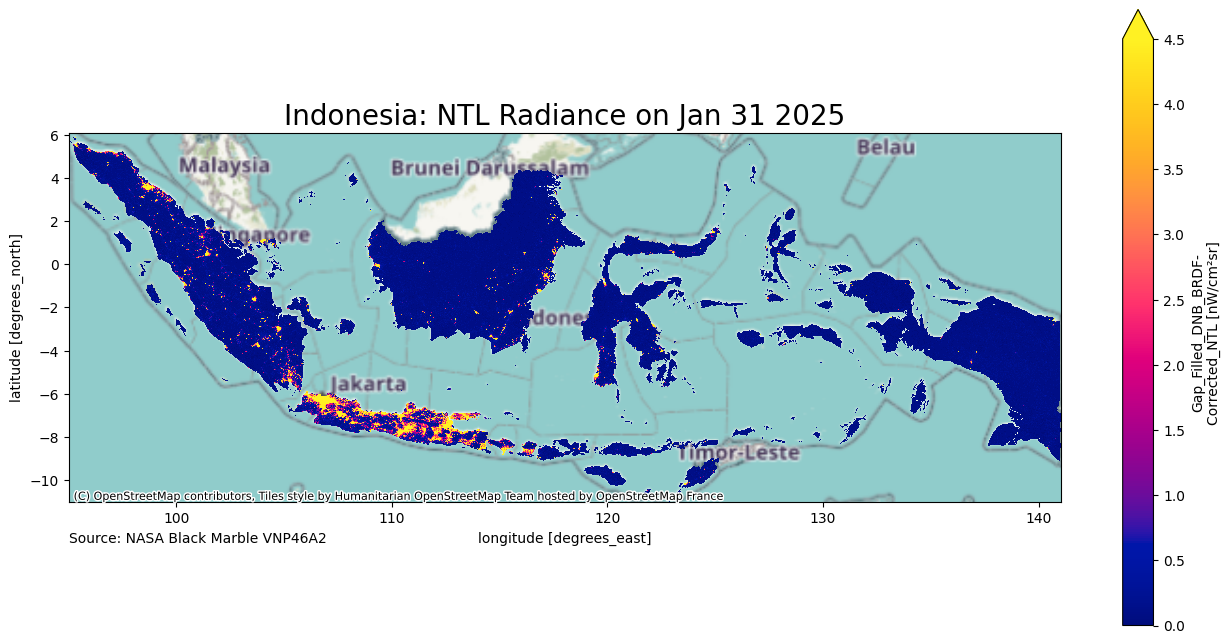
\includegraphics[keepaspectratio]{fig/nitelite.png}}

}

\caption{\label{fig-1}Annual Nighttime Lights in Indonesia, 2023}

\end{figure}%

Figure~\ref{fig-1} The figure is a visualization of the yearly raster
for nighttime lights in Indonesia in 2023. There is a stark contrast
between the nighttime lights activity in Java compared to other islands,
which is reflective of significant gaps in various socioeconomic
indicators between Java and the rest of Indonesia. The stark difference
in economic activity between Java and the rest of Indonesia is
well-documented in literature, and is a consequence of the landscape and
soil of the island facilitating stronger agricultural yields and
population growth.

Black Marble data can also be extracted for multiple time periods. The
function will return a raster stack, where each raster band corresponds
to a different date. The following code snippet provides examples of
getting data across multiple days, for the month of May 2024 in
Indonesia. We define a date range using pd.date\_range.

\begin{figure}

\centering{

\pandocbounded{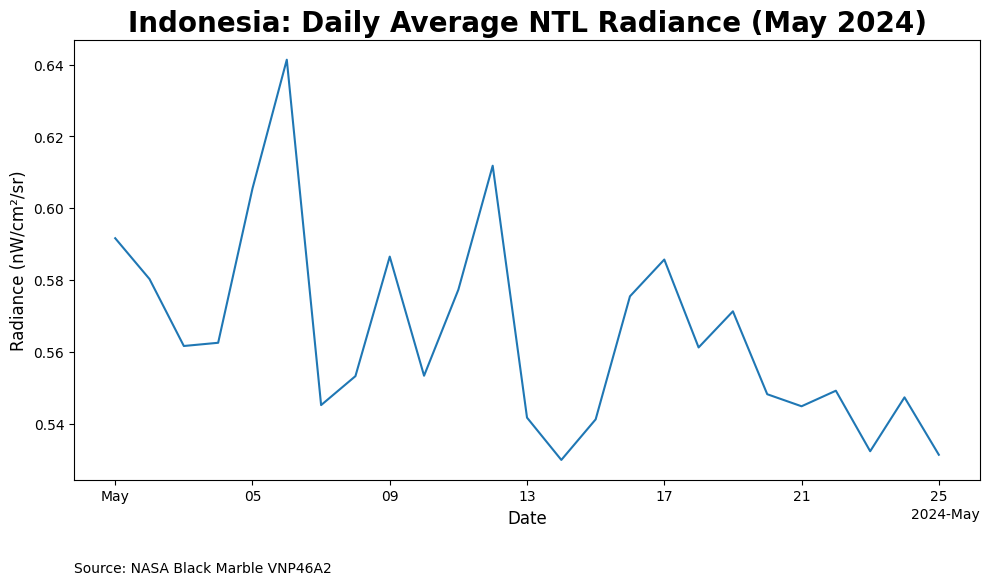
\includegraphics[keepaspectratio]{fig/file_show.png}}

}

\caption{\label{fig-may}Daily Average Nighttime Light Radiance in
Indonesia, May 2024}

\end{figure}%

Here we can see the fluctuations that exist within a given month,
fluctuations that may be difficult to pinpoint from monthly or yearly
rasters. One advantage of the flexibility of nighttime lights data is
the ability to process it to suit the needs of any kind of time series
analysis. In this instance, to facilitate the goal of making a proper
comparison between nighttime lights and GDP, both series needed to be
expressed on the same unit level. In Indonesia, GDP growth is typically
reported in quarterly year-on-year terms. To align the nighttime lights
data with this format, multiple steps were needed. First, monthly
rasters were extracted from January 2012 to December 2024, covering the
full period of available Black Marble nighttime lights data. The data
was then saved as a .zip file. The radiance values were also extracted
and saved as a separate .csv file.

With the radiance values extracted in a monthly form, the next steps
involved transforming the data into quarterly year-on-year terms.
Nighttime lights data was aggregated into quarterly terms. The data was
then lagged and shifted 1 year back, from which the year-on-year change
was able to be calculated.

GDP growth data was straightforward to collect due to the data being
readily available from the BPS website (BPS 2025). Quarterly GDP growth
from consumption side and aggregate GDP growth was used for the purposes
of this study. The GDP series includes data from Q1-2010 to Q2-2025, but
we will use Q1-2012 as our starting point in line with the availability
of nighttime lights data from NASA Black Marble.

\begin{figure}

\centering{

\pandocbounded{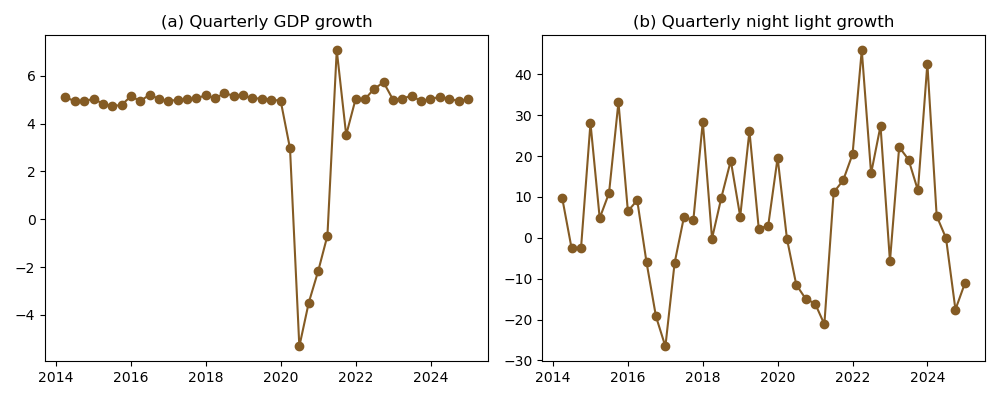
\includegraphics[keepaspectratio]{fig/fig.png}}

}

\caption{\label{fig-2}Indonesian economic growth and night light growth}

\end{figure}%

Figure~\ref{fig-2} shows our two main variables. The left panel is the
GDP growth sourced from BPS (2025) while the right panel is the
calculated night lights we gathered via Black Marble python package.
Both seems to follow similar trend. The pearson correlation for the two
vaariables is 0.44 which suggests a potential cointegration. However,
night light index doesn't show significant drop during the COVID time,
unlike the GDP growth.

Moreover, the volatility of the nighttime lights series could indicate
that there is no stable mean and that variance is constantly changing.
From the eye-test, it would appear that the series is non-stationary.
GDP growth, on the other hand, appears mostly stable outside of a large
structural break during the COVID period. This normally indicates the
series is stationary, but the structural break could cause potential
problems for formal models. An ADF test is needed to confirm the
stationarity of both series.

\section{Methodology}\label{methodology}

Unlike Henderson, Storeygard, and Weil (2012) and others, our dataset
does not contain any cross-sectional variation. Therefore, techniques
that utilise cross-sectional mean cannot be exploited. Multivariate time
series techniques, thus, should be the appropriate method.

Given the nature of the data as multivariate time series, certain tests
need to be performed before moving on to the modeling process (Enders
2014; Shrestha and Bhatta 2018). First, we check stationarity using the
ADF test to determine whether the two series are stationary at the same
level. Growth data are usually stationary for level variables. If the
series are truly stationary, Vector AutoRegression (VAR) would be the
most appropriate model choice. However, the structural breaks
experienced during COVID-19 could create potential problems due to shock
and scarring effects. There is a possibility of cointegration existing
between the two series. In such a case, the Vector Error Correction
Model (VECM) is the appropriate method to use. (Enders 2014; Shrestha
and Bhatta 2018).

\begin{figure}

\centering{

\pandocbounded{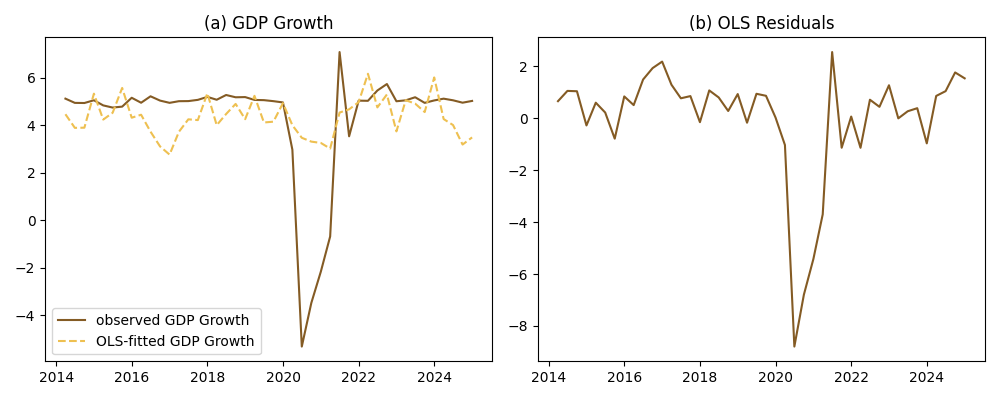
\includegraphics[keepaspectratio]{fig/ols.png}}

}

\caption{\label{fig-3}OLS fit and the residuals}

\end{figure}%

The ADF test shows that while the nighttime lights series is stationary,
the GDP growth series is not. We cannot reject the null hypothesis of
non-stationarity of the GDP growth series at the 5\% level. This is
contrary to typical growth number, potentially amid covid. It is
important to note that the p-value is pretty close to a rejection. This
suggestst that a structural VAR model model may still suitable if we
control for the COVID variable. Lastly, the potency that the two series
integrate at a different level also warrants the use of ARDL (Shrestha
and Bhatta 2018; Enders 2014).

We then proceed to the Johansen cointegration test. We first find a
proper lag, then proceed to the Johansen cointegration test.

\begin{table}

\caption{\label{tbl-1}Lag order selection for VECM}

\centering{

\begin{verbatim}
 VECM Order Selection (* highlights the minimums) 
==================================================
       AIC         BIC         FPE         HQIC   
--------------------------------------------------
0        7.151      7.507*      1278.*      7.274*
1        7.323       7.857       1526.       7.507
2        7.440       8.151       1731.       7.685
3        7.197       8.086       1380.       7.504
4        7.099       8.166       1283.       7.468
5        7.201       8.446       1474.       7.631
6        7.371       8.793       1839.       7.862
7        7.195       8.795       1656.       7.747
8        7.376       9.153       2183.       7.989
9        7.068       9.023       1825.       7.743
10       6.834       8.967       1721.       7.571
11       6.513       8.824       1585.       7.310
12      6.450*       8.938       2088.       7.309
--------------------------------------------------
\end{verbatim}

}

\end{table}%

Table~\ref{tbl-1} shows the results of lag selection method using AIC,
BIC, FPE and HQIC, all standard \texttt{statsmodel} procedure. All but
AIC point us to use 0-order VECM. Here, we test using AIC\footnote{We
  tried using the BIC-chosen lag but the fit is inferior to AIC-chosen
  lag.}.

Now that we have the order, we test whether the two series cointegrate
by running a standard Johansen Cointegration test.

\begin{table}

\caption{\label{tbl-2}Johansen Cointegration test}

\centering{

\begin{verbatim}
Johansen cointegration test using trace test statistic with 5% significance level
=====================================
r_0 r_1 test statistic critical value
-------------------------------------
  0   2          21.27          15.49
  1   2          6.971          3.841
-------------------------------------
\end{verbatim}

}

\end{table}%

Table~\ref{tbl-2} shows the results of our cointegration test. The null
hypothesis is there is no cointegration among variables used. The trace
test statistic results are larger than the critical value, which suggest
that we reject the null hypothesis. This would suggests a VECM as a
method of choice. However, the null hypothesis of the number of rank
equals two is also rejected. This suggests a potentially feasible two
cointegration equations. An equal number between the cointegration
equations and the endogeneous variables mean the VECM may perform no
different than VAR.

The ADF test and the Johanse cointegration test are not terribly
conclusive, we proceed with testing three potential multivariate time
series technique, namely VAR, ARDL and VECM. To sum up:

\begin{itemize}
\item
  VECM reasons: Both are not integrated at the same level, OLS-residuals
  is stationary, Johansen Cointegration failed to reject \(H_0\).
\item
  VAR reasons: Economic growth is \emph{almost} stationary (p-value is
  very close to the critical level), Johansen Cointegration failed to
  reject a possibility of only 1 cointegration coefficient.
\item
  ARDL reason: Economic growth \(I(1)\) while the night light growth is
  \(I(0)\). Additionally, ARDL allows for one endogeneous
  variable\footnote{As discussed above, previous papers use
    cross-sectional regression which presents no lag. Night light is
    also more immune from administrative error and other kinds of
    potential biases.}.
\end{itemize}

For robustness, we also try to do the time series on the log quarterly
GDP and night light instead of growth.

\section{Results and discussions}\label{results-and-discussions}

We ran various specifications, including dummy quarterly, dummy COVID
(2020-2022), and dummy scarrin (2020 onwards). Additionally, we also
tried various lag specifications, including BIC-selected lags and
HQ-selected lags. In this paper, we show results from the no dummy and
dummy scarring using AIC-selected lags amid the most consistent. We show
all VECM, VAR and ARDL models. We also only show graph in this section
because we concern mostly on fitting the model at this stage of
reasearch. Regression table and some explanations are at the appendix.

\subsection{Growth regression}\label{growth-regression}

\subsubsection{VECM}\label{vecm}

\pandocbounded{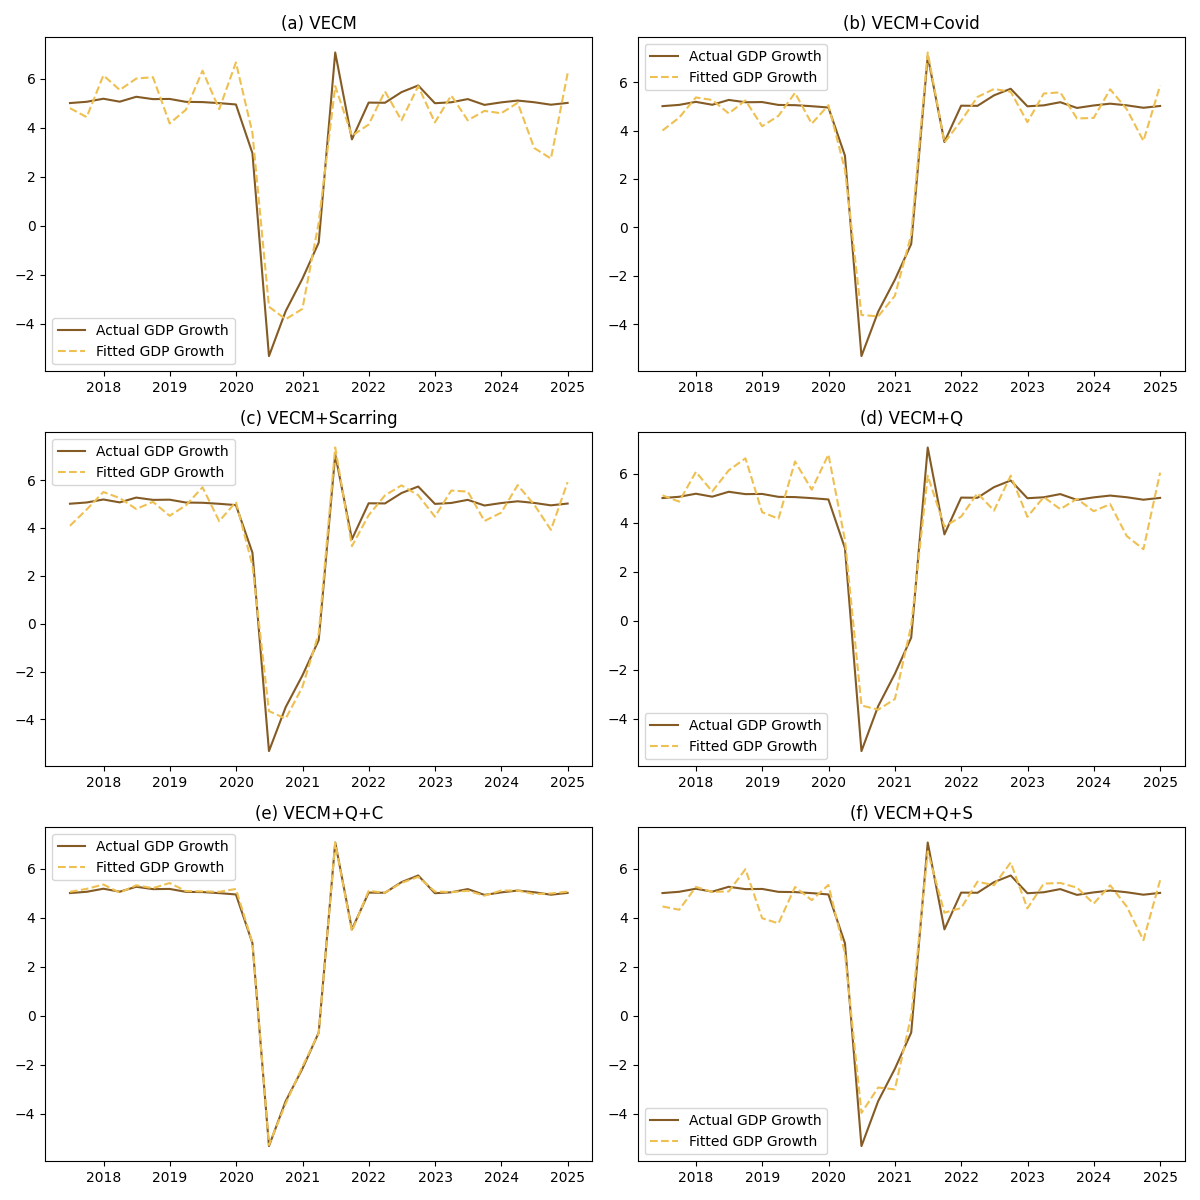
\includegraphics[keepaspectratio]{fig/VECM.png}}

\subsubsection{VAR}\label{var}

\pandocbounded{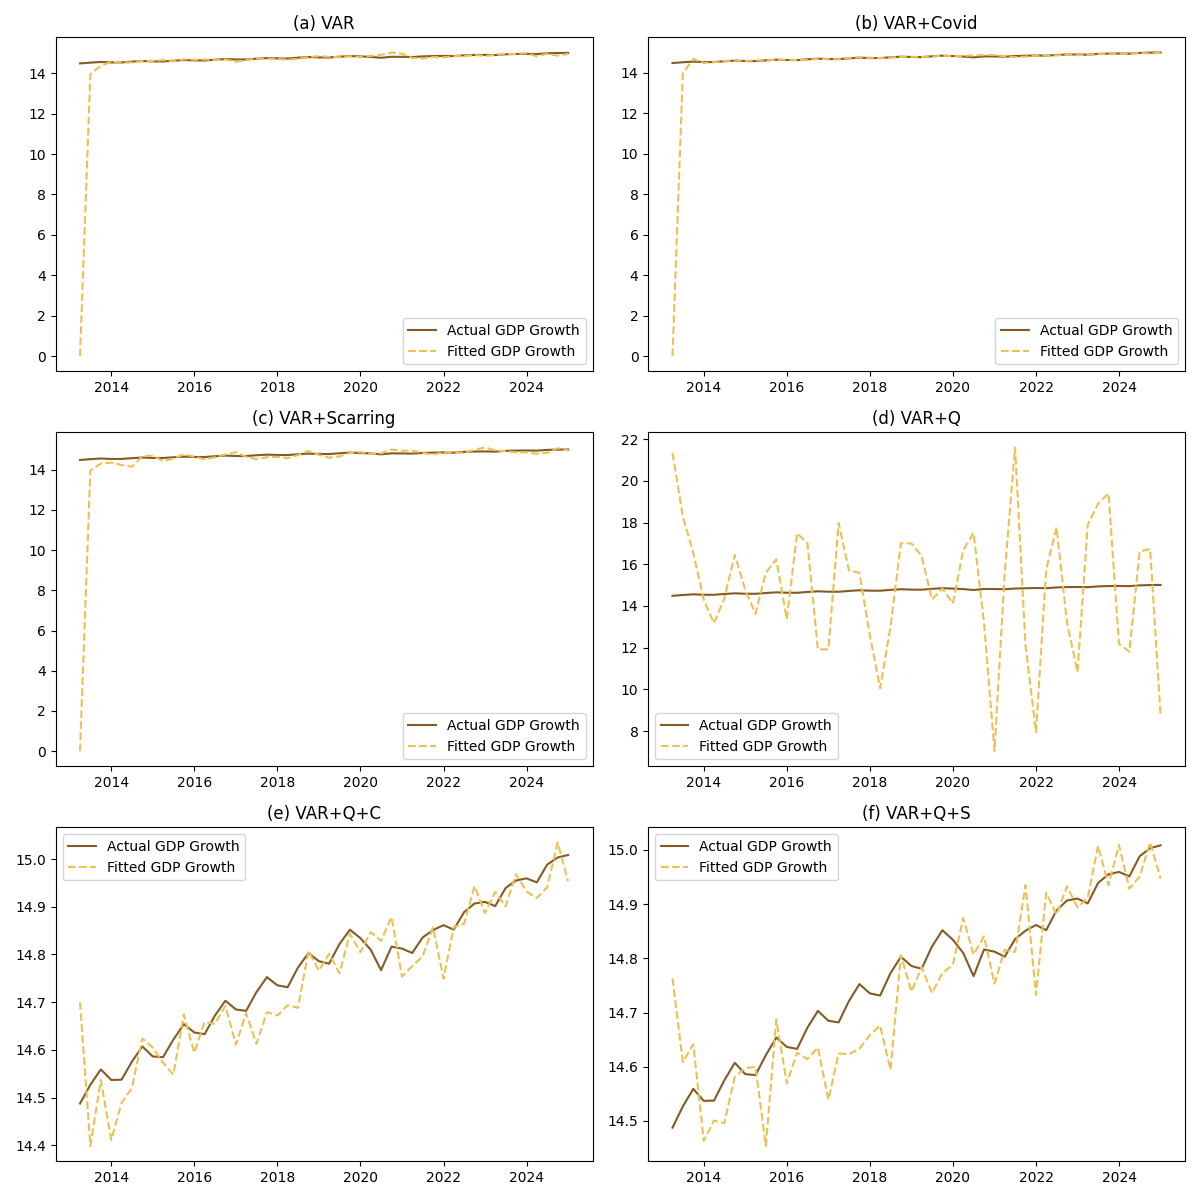
\includegraphics[keepaspectratio]{fig/VAR.png}}

\subsubsection{ARDL}\label{ardl}

\pandocbounded{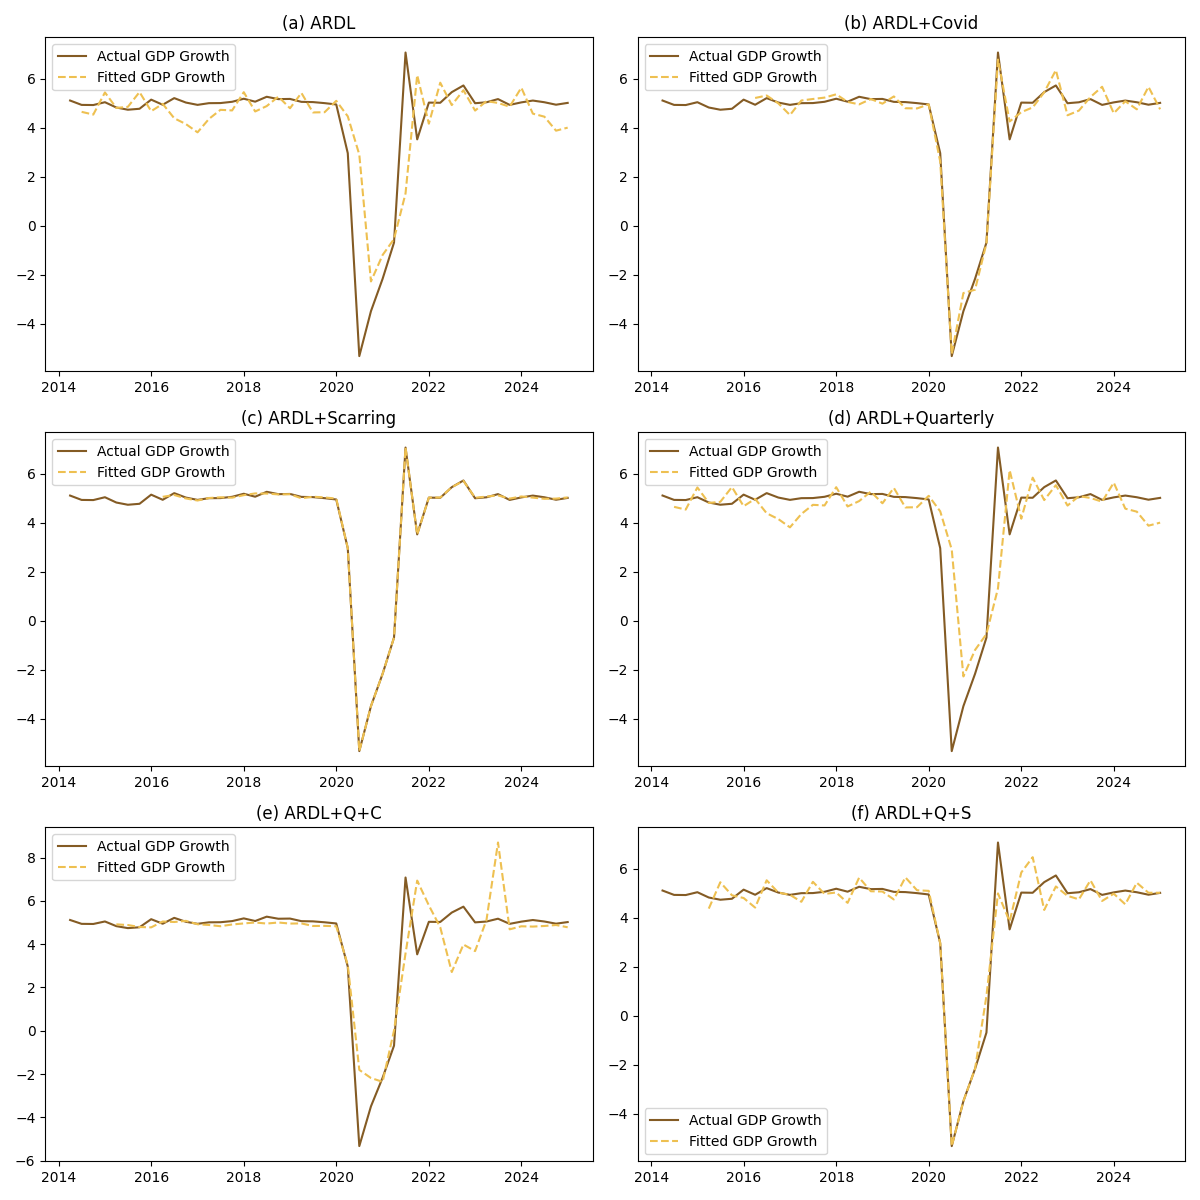
\includegraphics[keepaspectratio]{fig/ARDL.png}}

\subsection{Quarterly regression}\label{quarterly-regression}

\pandocbounded{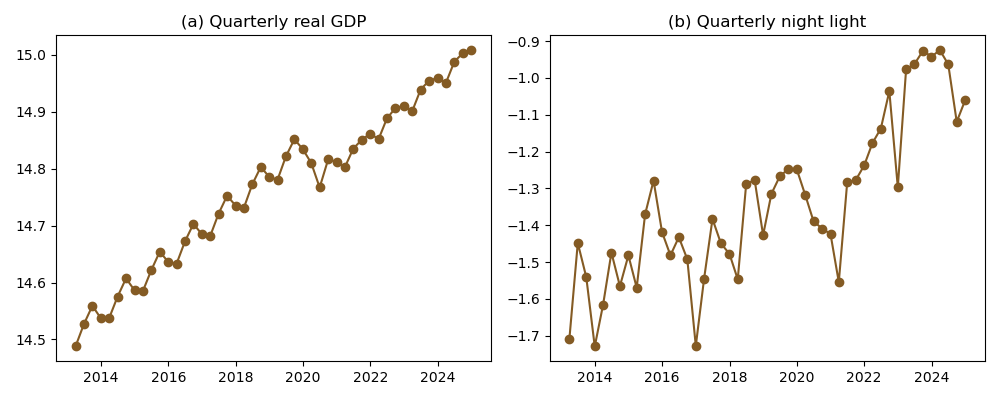
\includegraphics[keepaspectratio]{fig/figQ.png}}

\pandocbounded{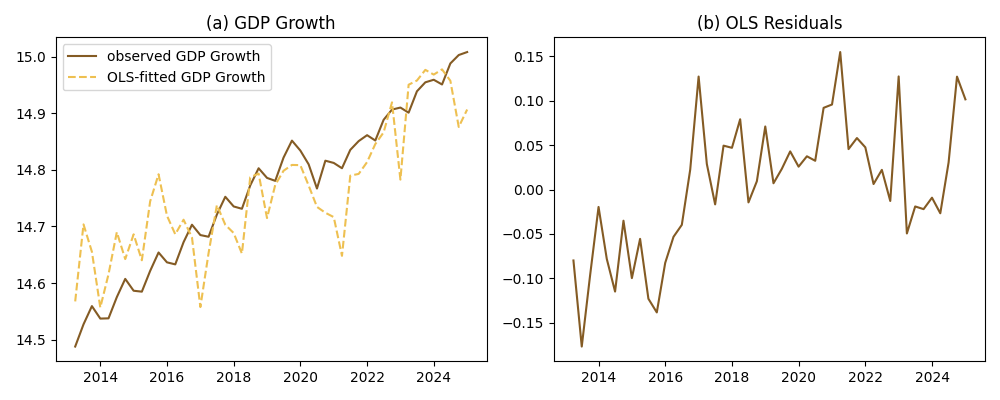
\includegraphics[keepaspectratio]{fig/Qols.png}}

\subsubsection{VECM}\label{vecm-1}

\pandocbounded{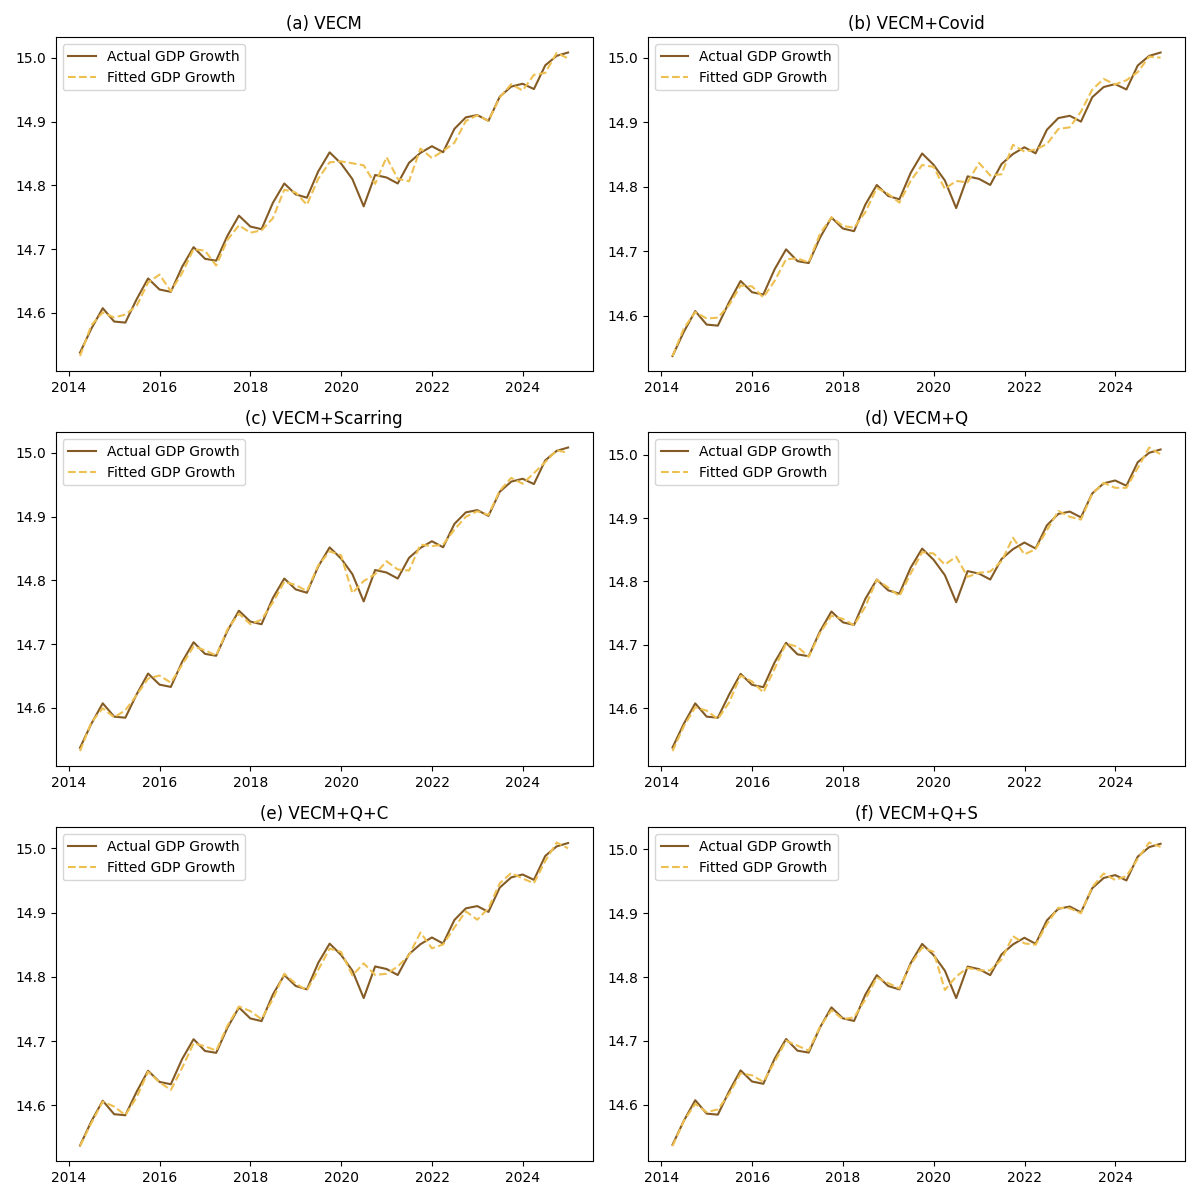
\includegraphics[keepaspectratio]{fig/VECMQ.png}}

\subsubsection{ARDL}\label{ardl-1}

\pandocbounded{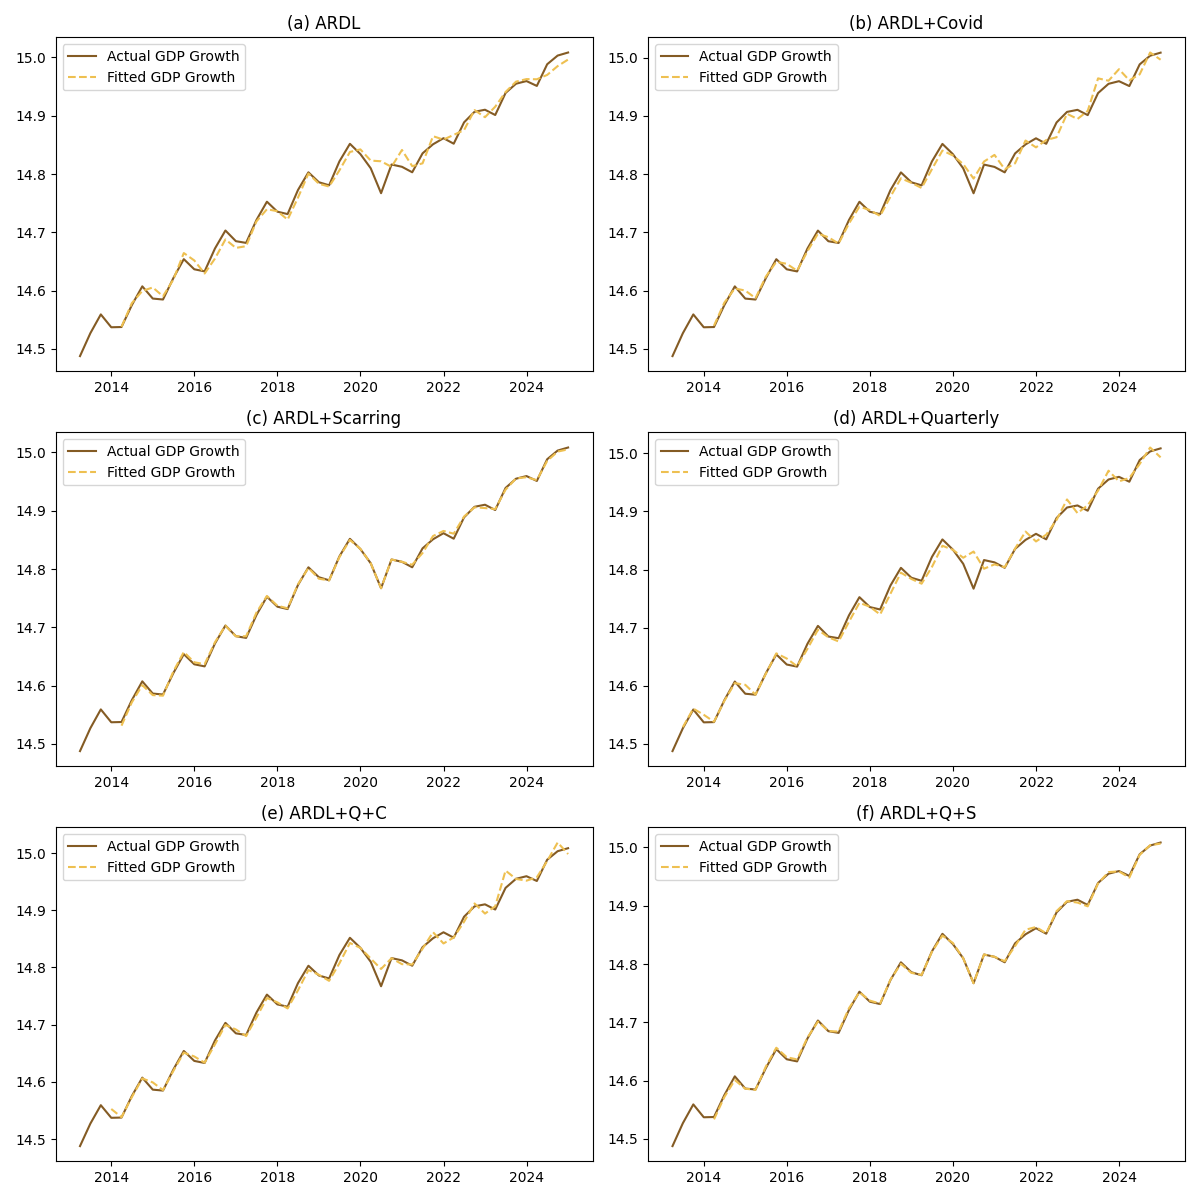
\includegraphics[keepaspectratio]{fig/ARDLQ.png}}

\section{Conclusion}\label{conclusion}

\section*{References}\label{references}
\addcontentsline{toc}{section}{References}

\phantomsection\label{refs}
\begin{CSLReferences}{1}{1}
\bibitem[\citeproctext]{ref-nl2}
Bickenbach, Frank, Eckhardt Bode, Peter Nunnenkamp, and Mareike Söder.
2016. {``Night Lights and Regional GDP.''} Journal Article. \emph{Review
of World Economics} 152 (2): 425--447.
https://doi.org/\url{https://doi.org/10.1007/s10290-016-0246-0}.

\bibitem[\citeproctext]{ref-bps}
BPS. 2025. \emph{{[}Seri 2010{]} 4. Laju Pertumbuhan PDB Menurut
Pengeluaran, 2025. Diakses Pada 14 September 2025}.
Https://www.bps.go.id/id/statistics-table/2/MTA4IzI=/-seri-2010--4--laju-pertumbuhan-pdb-menurut-pengeluaran--persen-.html.

\bibitem[\citeproctext]{ref-enders}
Enders, Walter. 2014. \emph{Applied Econometric Time Series}. Wiley.

\bibitem[\citeproctext]{ref-nle}
Gibson, John, Susan Olivia, and Geua Boe-Gibson. 2020. {``Night Lights
in Economics: Sources and Uses.''} Journal Article. \emph{Journal of
Economic Surveys} 34: 955--980.
https://doi.org/\url{https://doi.org/10.1111/joes.12387}.

\bibitem[\citeproctext]{ref-nl}
Henderson, J. Vernon, Adam Storeygard, and David N. Weil. 2012.
{``Measuring Economic Growth from Outer Space.''} \emph{The American
Economic Review} 102 (2): 994--1028.
\url{http://www.jstor.org/stable/23245442}.

\bibitem[\citeproctext]{ref-nl3}
Martínez, Luis R. 2022. {``How Much Should We Trust the Dictator's GDP
Growth Estimates?''} Journal Article. \emph{Journal of Political
Economy} 130 (10): 2731--2769. \url{https://doi.org/10.1086/720458}.

\bibitem[\citeproctext]{ref-ts}
Shrestha, Min B., and Guna R. Bhatta. 2018. {``Selecting Appropriate
Methodological Framework for Time Series Data Analysis.''} Journal
Article. \emph{The Journal of Finance and Data Science} 4 (2): 71--89.
https://doi.org/\url{https://doi.org/10.1016/j.jfds.2017.11.001}.

\bibitem[\citeproctext]{ref-blackmarblepy}
Stefanini Vicente, Gabriel, and Robert Marty. 2023.
\emph{{BlackMarblePy: Georeferenced Rasters and Statistics of Nighttime
Lights from NASA Black Marble}}.
\href{https://worldbank.github.io/blackmarblepy}{Https://worldbank.github.io/blackmarblepy}.
\url{https://doi.org/10.5281/zenodo.10667907}.

\end{CSLReferences}

\section{Appendix}\label{appendix}

\section*{Appendix A}\label{appendix-a}
\addcontentsline{toc}{section}{Appendix A}




\end{document}
